\chapter{Multisample Anti Aliasing}

If we examine up close the images we have rendered up to this point, we
can notice that some of our edges have a jagged saw like pattern.
This effect is called aliasing and it's the result of having to render our
images on a grid with a finite number of pixels.
We can't completely avoid this effect since screens will always have a
finite resolution.
We can, however, attenuate the issue using a technique known as multisample
anti aliasing, MSAA for short.

\begin{figure}[H]
    \centering
    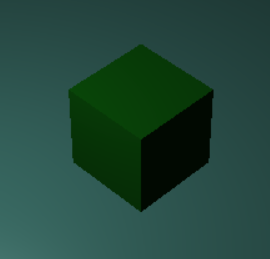
\includegraphics[scale=1.0]{images/ChMSAA/AnExampleOfAliasing.png}
    \caption{An example of aliasing}
    \label{fig::AliasingExample}
\end{figure}

\section{MSAA}

So far, we have always used only one sample per pixel.
This means that we determine its color using a single sample
point, placed at its center.
If the rendered geometry doesn't cover the sample point, the entire pixel
is left blank.
Else, if the rendered geometry covers the sample point, we color the entirety of
the pixel.
This is what causes aliasing.

\begin{figure}[H]
    \centering
    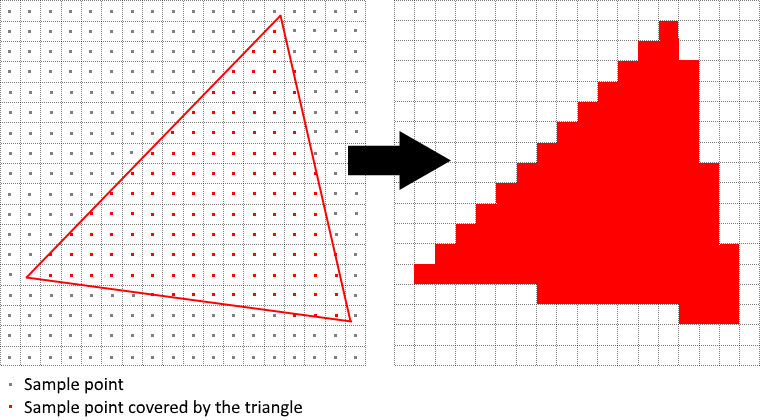
\includegraphics[scale=0.6]{images/ChMSAA/OneSamplePerPixel.png}
    \caption{Rendering using one sample per pixel}
    \label{fig::OneSamplePerPixel}
\end{figure}

\begin{figure}[H]
    \centering
    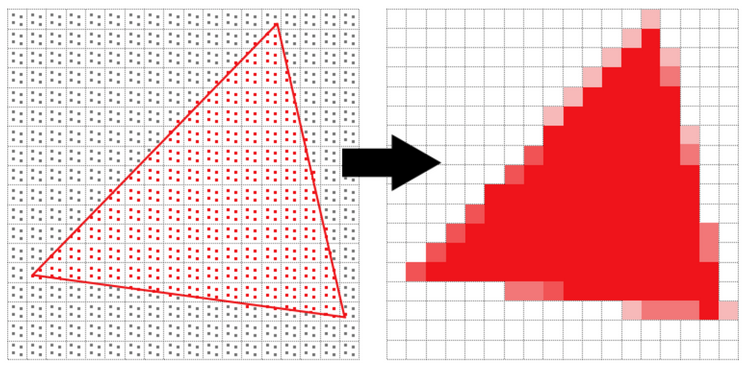
\includegraphics[scale=0.62]{images/ChMSAA/FourSamplesPerPixel.png}
    \caption{Rendering using four samples per pixel}
    \label{fig::FourSamplesPerPixel}
\end{figure}

MSAA uses multiple sample points per pixel to determine its final color.
More samples lead to better results but also mean more overhead.
For each pixel, the less the samples are covered by the geometry, the less
the geometry color contributes to the pixel final color.
Thanks to this, edges are surrounded by colors slightly lighter than the
edge's color itself.
This causes the edge to appear smooth when viewed from a distance.

\section{Adding MSAA In Vulkan}

In this section we discuss all the steps that are necessary to add MSAA
to our Vulkan application.

\subsection{Get Available Sample Count}

We must determine how many samples our hardware can use.
To do this we query the maximum number of samples for both color and depth values.
After that, we pick the highest sample count that they both support.

\begin{minipage}{\linewidth}{\noindent}
    \lstinputlisting[
        language=C++,
        caption={Determine the maximum supported sample count},
        label={lst::GetMaxMSAASampleCount}
        ]{src/ChMSAA/GetMaxMSAASampleCount.cpp}
\end{minipage}

\subsection{Create New Render Target}

Up to this point, we have always used the next swapchain image as our
render target.
The problem is that our swapchain images store only one sample per pixel.
They can't store more than one sample per pixel, because that, would make
them not presentable.
Thus, we have to create a new multisampled image that will be used
as our application's render target.

\subsubsection{Creating The Multisample Render Target}

To create our new render target, we reuse the image creation functions
we saw in earlier chapters.
The only thing different from before, is that we now pass the
number of samples that our image will store per pixel.

\begin{minipage}{\linewidth}{\noindent}
    \lstinputlisting[
        language=C++,
        caption={Create the multisample render target},
        label={lst::CreateMultisampleRenderTarget}
        ]{src/ChMSAA/CreateMultisampleRenderTarget.cpp}
\end{minipage}

\subsubsection{Update Depth Buffer Creation}

We must also remember to update the depth buffer creation.
This is because the depth buffer will also store more samples per pixel.

\subsection{Update Render Pass}

We set the color attachment and the depth attachment samples count
to \texttt{msaaSamples}.
We also change the color attachment's final layout to
\texttt{VK\_IMAGE\_LAYOUT\_COLOR\_ATTACHMENT\_OPTIMAL}.
We do this because multisampled images can't be directly presented.

\subsubsection{Add A Resolve Color Attachment}

Right now, we only have a multisampled render target and a multisampled
depth buffer.
Neither is suitable to be presented to the screen.
Because of this, we add a new color attachment to the render pass.
After finishing our rendering operations, we will resolve our render target to
this new color attachment.
This resolve color attachment is the one that will be presented to the screen.

\begin{minipage}{\linewidth}{\noindent}
    \lstinputlisting[
        language=C++,
        caption={Color resolve attachment},
        label={lst::ColorResolveAttachment}
        ]{src/ChMSAA/ColorResolveAttachment.cpp}
\end{minipage}

\subsubsection{Render Pass Attchments}

Now our render pass has three attachments.

\begin{minipage}{\linewidth}{\noindent}
    \lstinputlisting[
        language=C++,
        caption={MSAA render pass attachments},
        label={lst::MSAARenderPassAttachments}
        ]{src/ChMSAA/MSAARenderPassAttachments.cpp}
\end{minipage}

\subsubsection{Update Color Subpass Description}

We must tell to our color subpass to actually use the color resolve attachment.
To do this we update its description.

\begin{minipage}{\linewidth}{\noindent}
    \lstinputlisting[
        language=C++,
        caption={Color resolve attachment reference},
        label={lst::ColorResolveAttachmentReference}
        ]{src/ChMSAA/ColorResolveAttachmentReference.cpp}
\end{minipage}

\subsection{Update Multisampling Pipeline State}

Not only we need to create resources that are compatible with MSAA.
We also need to directly enable it while creating the pipeline state object.

\begin{minipage}{\linewidth}{\noindent}
    \lstinputlisting[
        language=C++,
        caption={Enable multisampling},
        label={lst::MSAAPipelineMultisampleState}
        ]{src/ChMSAA/MSAAPipelineMultisampleState.cpp}
\end{minipage}

\subsection{Update Framebuffer}

Now that we have updated our render pass attachments, we also must update
the attachments that are used by our framebuffers.
We use the multisample render target as the first attachment.
We use the depth buffer as the second attachment.
And we use the next swapchain image as the color resolve attachment.

\section{Side By Side Comparison}

Here we can see a side by side comparison of how MSAA influences the
rendered image's quality.
On the left we see the cube rendered without using MSAA.
On the right we see the cube rendered using MSAA.
As explained earlier, the jagged pattern gets blurred making it look
smoother.
This leads to more pleasant visuals.

\begin{figure}[H]
    \centering
    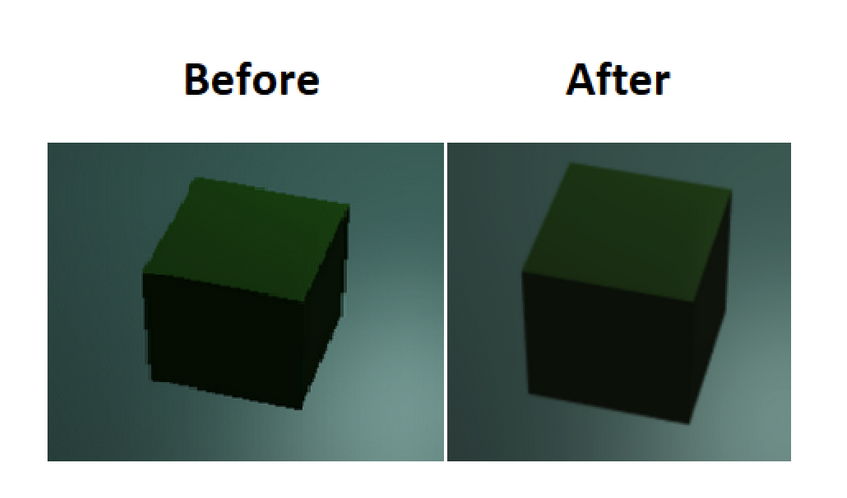
\includegraphics[scale=0.40]{images/ChMSAA/BeforeAfterMSAA.png}
    \caption{Before and after MSAA}
    \label{fig::MSAASideBySide}
\end{figure}
